\hypertarget{recurrent-quantum-neural-networks}{%
\section{Recurrent Quantum Neural
Networks}\label{recurrent-quantum-neural-networks}}

\hypertarget{introduction}{%
\subsection{Introduction}\label{introduction}}

The project is driven by the absence of any viable recurrent quantum
network. Although Variational Quantum Eigensolvers (VQEs) exist, the
resultant Quantum Circuits are very dense, compressing a lot of
parameters into a relatively compact circuit
\protect\hyperlink{quantum-neuron-an-elementary-building-block-for-machine-learning-on-quantum-computers}{{[}1{]}}.
The high density of entangling gates, lack of correlation between
parameters results in highly over-parameterized models which are hard to
train on classification tasks on inputs larger than a few bits.

This project focusses on constructing a QRNN, and compare it's
performance on non-trivial tasks such as sequence learning and integer
digit classification.

The reference paper exploits the nature of quantum mechanics. The
interatcions of any quantum system can be described by a Hermitian
Operator \(\bold{\mathcal{H}}\) which generates the system's time
evolution under the unitary map: \[U(t) = \exp(-itH)\] which is a
solution to the Schrodinger equation.

Further, any quantum circuit compresing a sequence of individual unitary
quantum gates of the form \(U_i(t_i)\) for a set of parameters \(t_i\)
is intrinsically unitary and inherently linear
\protect\hyperlink{recurrent-quantum-neural-networks-1}{{[}1{]}}. This
is promising because then a parameterized quantum circuit serves as a
prime candidate for a unitary recurrent network.

\hypertarget{qnlp}{%
\subsection{QNLP}\label{qnlp}}

We start with experiments on Quantum Natural Language Processing. This
represents a fascination convergence between quantum computing and
computational linguistics, aimed at enhancing natural language
processing (NLP) tasks. We start off with a simple integration of lambeq
and Pennylane libraries.

The setup for the hybrid QNLP model involves defining training dataset,
which includes sentence pairs labeled according to their topical
relevance. We try creating a hybrid model, trained to perform XOR
operations on the outputs to discern if the sentences share the same
topic. Upon training, hte model demonstrates a clear capacity to
differentiate between topics, achieving perfect accuracy on the
development set and showcasing effective internal representation within
quantum circuits.

\hypertarget{qrnn-cell-and-network}{%
\subsection{QRNN Cell and Network}\label{qrnn-cell-and-network}}

The fundamental building block is an improved type of quantum neuron
based to introduce non-linearity
\protect\hyperlink{recurrent-quantum-neural-networks-1}{{[}2{]}}. In
addition, we employ a type of fixed-point amplitude amplification (done
during training) which alows the introduction of measurements. These
both operations remains arbitrarily close to unitary. This
implementation is the first quantum machine learning model capable of
working with non-superposed training data.

There are three parts of the QRNN cell. - The input stage, where at each
step, it writes the current input into the cell state - Multiple work
stages, where it computes with input and cell states - Final output
stage, which creates a probability density over possible predictions.

Although the resulting circuits are deeper than VQEs, it only requires
as many qubits as the input and cell states are wide.

The figures below show the QRNN Cell, and how it can be used to
construct a QRNN.

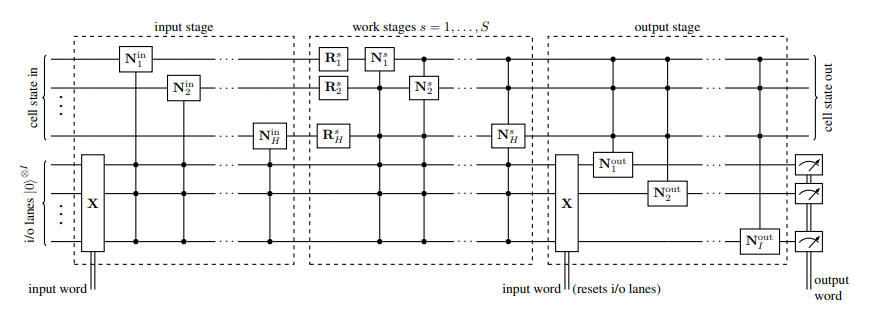
\includegraphics{./assets/QRNN_Cell.png} \[\textit{QRNN Cell}\]
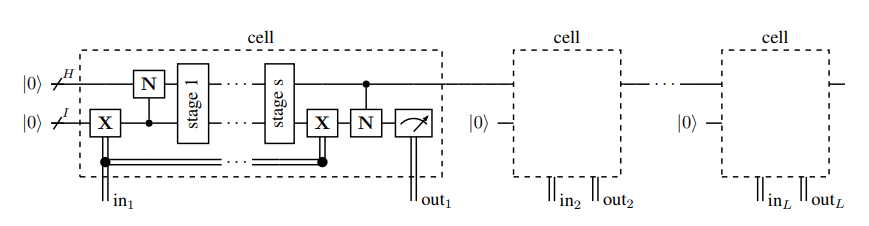
\includegraphics{./assets/QRNN.png} \[\textit{QRNN}\]

\hypertarget{implementation}{%
\subsection{Implementation}\label{implementation}}

\hypertarget{references}{%
\subsection{References}\label{references}}

\hypertarget{recurrent-quantum-neural-networks-bausch-j.}{%
\subparagraph{\texorpdfstring{\href{./references/2006.14619.pdf}{Recurrent
Quantum Neural Networks}, Bausch
J.}{Recurrent Quantum Neural Networks, Bausch J.}}\label{recurrent-quantum-neural-networks-bausch-j.}}

\hypertarget{quantum-neuron-an-elementary-building-block-for-machine-learning-on-quantum-computers-cao-y.-etal}{%
\subparagraph{\texorpdfstring{\href{./references/1711.11240.pdf}{Quantum
Neuron: an elementary building block for machine learning on quantum
computers}, Cao Y.
et,al}{Quantum Neuron: an elementary building block for machine learning on quantum computers, Cao Y. et,al}}\label{quantum-neuron-an-elementary-building-block-for-machine-learning-on-quantum-computers-cao-y.-etal}}
